\chapter{Нейросетевые модели управления технологическими процессами}

В данной главе рассматриваются практические примеры применения в задачах АСУТП.

\section{Процесс пастеризации молока}

\subsection{Общие сведения}

К концу XIX века тепловая обработка молока получила столь широкое применение, что стала использоваться для разнообразных целей на большинстве молокозаводов – например, для обработки молока при изготовлении сыра и масла. До внедрения тепловой обработки молоко представляло собой постоянный источник инфекций, так как оно является идеальной средой для развития микроорганизмов. Через молоко зачастую распространялись такие болезни, как туберкулез и брюшной тиф.

В термине “пастеризация” запечатлено имя Луи Пастера, который в середине XIX века провел фундаментальные исследования воздействия тепла на микроорганизмы, приводящего к их гибели, и возможности применения температурной обработки для консервирования пищевых продуктов.

Пастеризация молока – это особый вид тепловой обработки, который можно определить как “любую тепловую обработку молока, обеспечивающую безусловное уничтожение микроорганизмов – возбудителей туберкулеза, не вызывая при этом значительных изменений физических и химических качеств молока” \cite{TetraPak1995}.

Пластинчатая пастеризационно-охладительная установка (ПОУ) предназначена для тепловой обработки и охлаждения молочных продуктов в непрерывном тонкослойном закрытом потоке. Схема типовой пастеризационной установки приведена ниже (рис. \ref{fig:POU_Tetra_Pak}). Нагрев осуществляется за счет подачи пара через управляемый клапан \textbf{VC1}. Диапазон работы управляемых паровых клапанов от $\text{0\%}$ – полностью закрыт, до $\text{100\%}$ – полностью открыт. Температура \textbf{TE1} поддерживаться в пределах $92 \pm 2 \SI{}{\celsius}$.

Современная ПОУ, включающая оборудование для эксплуатации, надзора и управления процессом, собирается из согласованных компонентов, образуя сложный технологический агрегат. Для автоматизации регулирования температурного режима в состав ПОУ входит система управления на базе промышленного контроллера. От применяемых алгоритмов управления напрямую зависит качество получаемой продукции.

\begin{figure}[H]
    \centering
    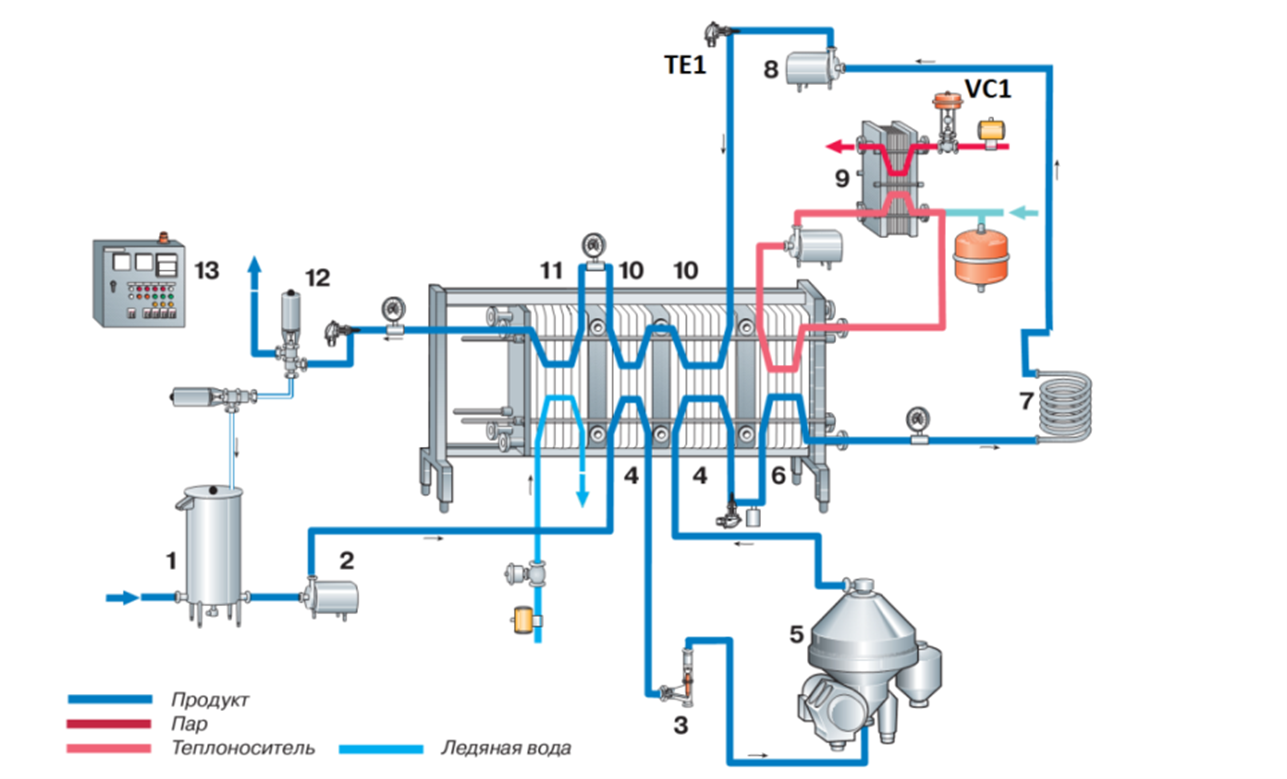
\includegraphics[width=\textwidth]{images/chapter_2/ПОУ Tetra Pak.png}
    \caption{Схема и общий вид пастеризационной установки, где: 1 - балансный танк, 2 - подающий насос, 3 - регулятор потока, 4 - секции регенеративного предварительного подогрева, 5 - центробежный очиститель, 6 - секция нагрева, 7 - труба выдержки, 8 - вспомогательный насос, 9 - система нагрева горячей воды, 10 - секции регенеративного охлаждения, 11 - секции охлаждения, 12 - клапан возвратный, 13 - панель управления}
    \label{fig:POU_Tetra_Pak}
\end{figure}

\subsection{Пастеризационные установки как объект автоматизации}

Рассмотрим подробно секцию нагрева ПОУ. Входные и выходные параметры и возмущающие воздействия для нее представлены на рис. \ref{fig:Pasterizer_heat_section}.

\begin{figure}[H]
    \centering
    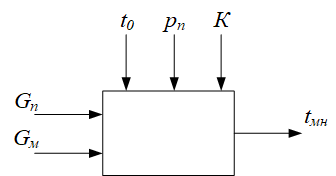
\includegraphics{images/chapter_2/Pasterizer_heat_section.png}
    \caption{Структурная схема секции нагрева ПОУ как объекта автоматизации}
    \label{fig:Pasterizer_heat_section}
\end{figure}

Таким образом, передаточная функция нагревательной части установки характеризуется последовательно соединенными апериодическим звеном первого порядка и звеном транспортного запаздывания. В таблице \ref{table:pasterizer_params} приведены средние значения параметров некоторых ПОУ.

\begin{table} [!h]
    \small
    \caption{Параметры ПОУ}\label{table:pasterizer_params}
    \centering
    \begin{tabular}{ | c | c | c | c | }
        \hline
        \textbf{Установка} & $K_\text{п}$, \SI{}{\celsius}/(кг/с) & $T$, c & $\tau_\text{з}$, c \\
        \hline
        ОПУ-5М             & 2300                                 & 369    & 12                 \\
        \hline
        ОПУ-10             & 1150                                 & 190    & 7                  \\
        \hline
        ОПУ-25             & 525                                  & 450    & 4                  \\
        \hline
    \end{tabular}
\end{table}
